\subsection*{ГЛ12 2}
\textbf{(а)}\\
Пусть инволюция $\sigma_1$ задается точкой $p_1$, неподвижные точки -- точки $a$ и $b$, а инволюция $\sigma_2$ задается точкой $p_2$,  неподвижные точки -- точки $c$ и $d$.\\
%Гармоничность двух пар точек $\{a, b\}$ и $\{c, d\}$ равносильна тому, что их двойное отношение не меняется при перестановке точек в одной из этих пар. 
\vskip 0.2in
\noindent
\textbf{Утверждение.} $\sigma_2(a)=b$ если и только если $[a,b,c,d]=-1$\\
\textbf{Доказательство.} Так как $[a,b,c,d]=[b,a,c,d]$, то $[a,b,c,d]^2=1$. Если $[a,b,c,d]=1$, то точки $a$ и $b$ совпадают, следовательно $\sigma = id$. тк инволюция нетривиальна, то $[a,b,c,d]=-1$.\\
аналогично  $\sigma_1(c)=d \Leftrightarrow [a,b,c,d]=-1$\\
\vskip 0.2in
\noindent
теперь докажем утверждение задачи 2а.\\
если: очевидно из рисунка\\
\begin{figure}[h!]
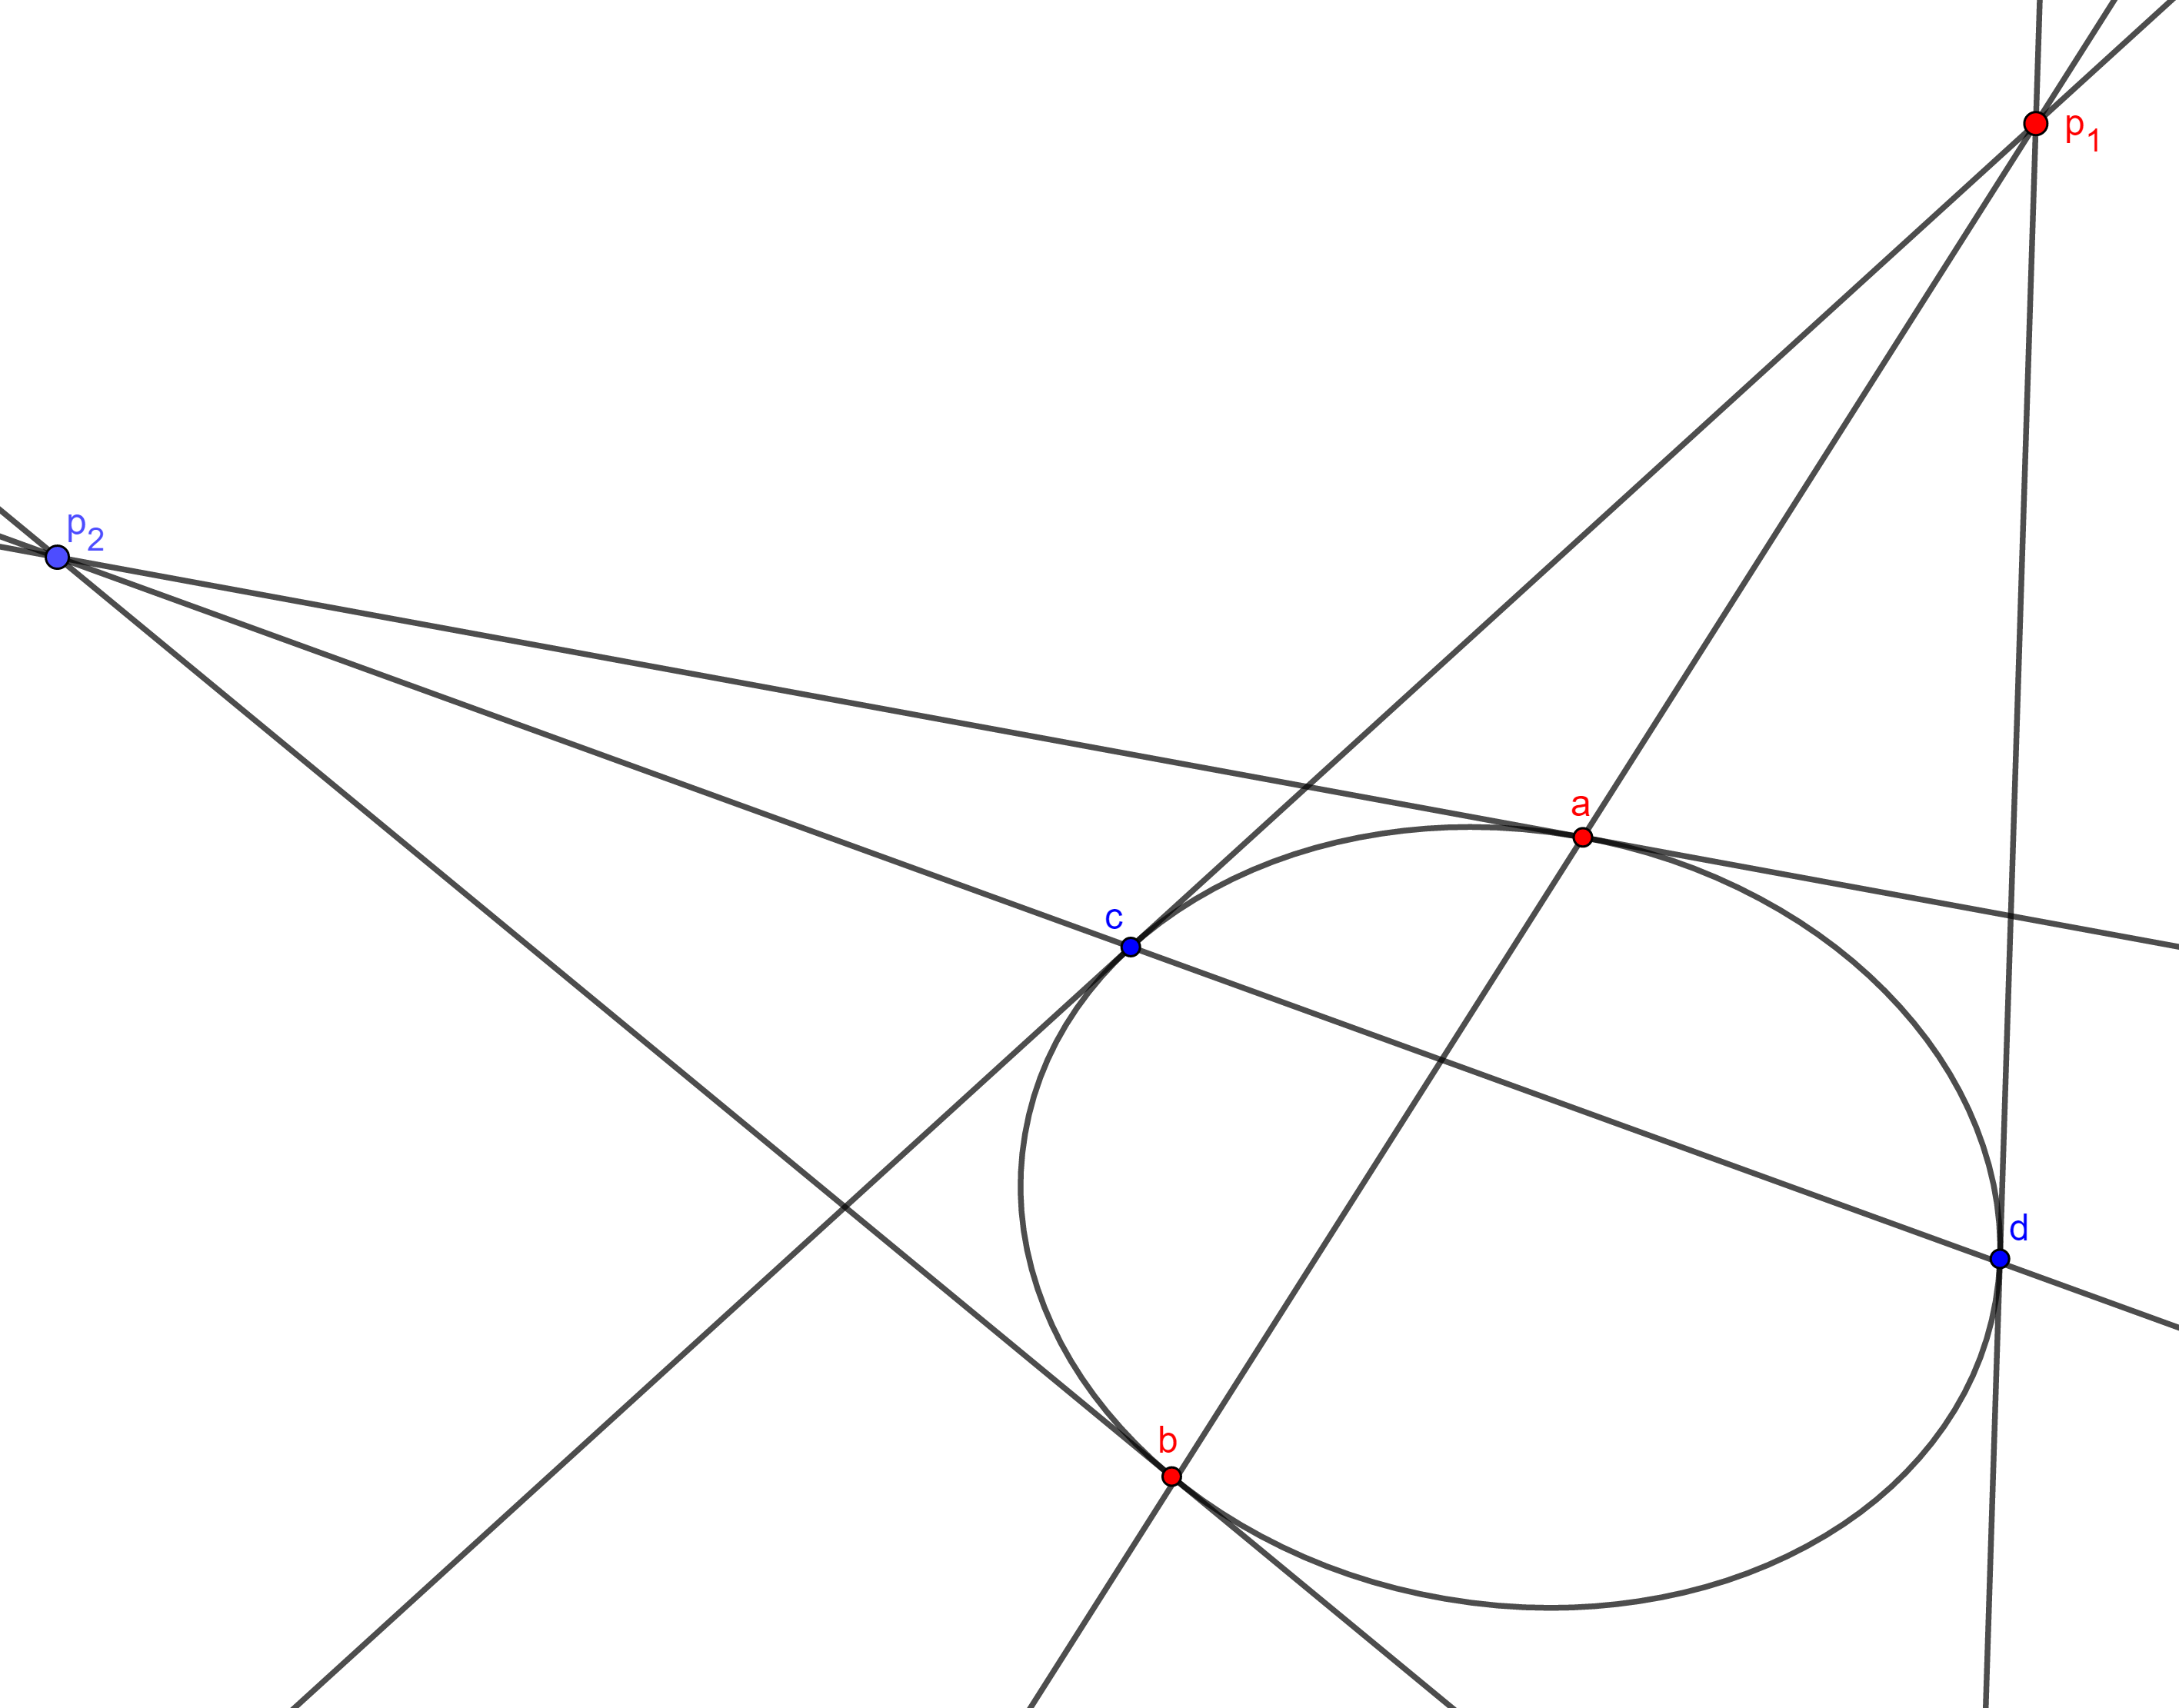
\includegraphics[width=0.5\linewidth]{pic18}
\end{figure}\\
только если:\\
спроецируем точки $a, b, c, d$ на прямую.\\
\begin{figure}[h!]
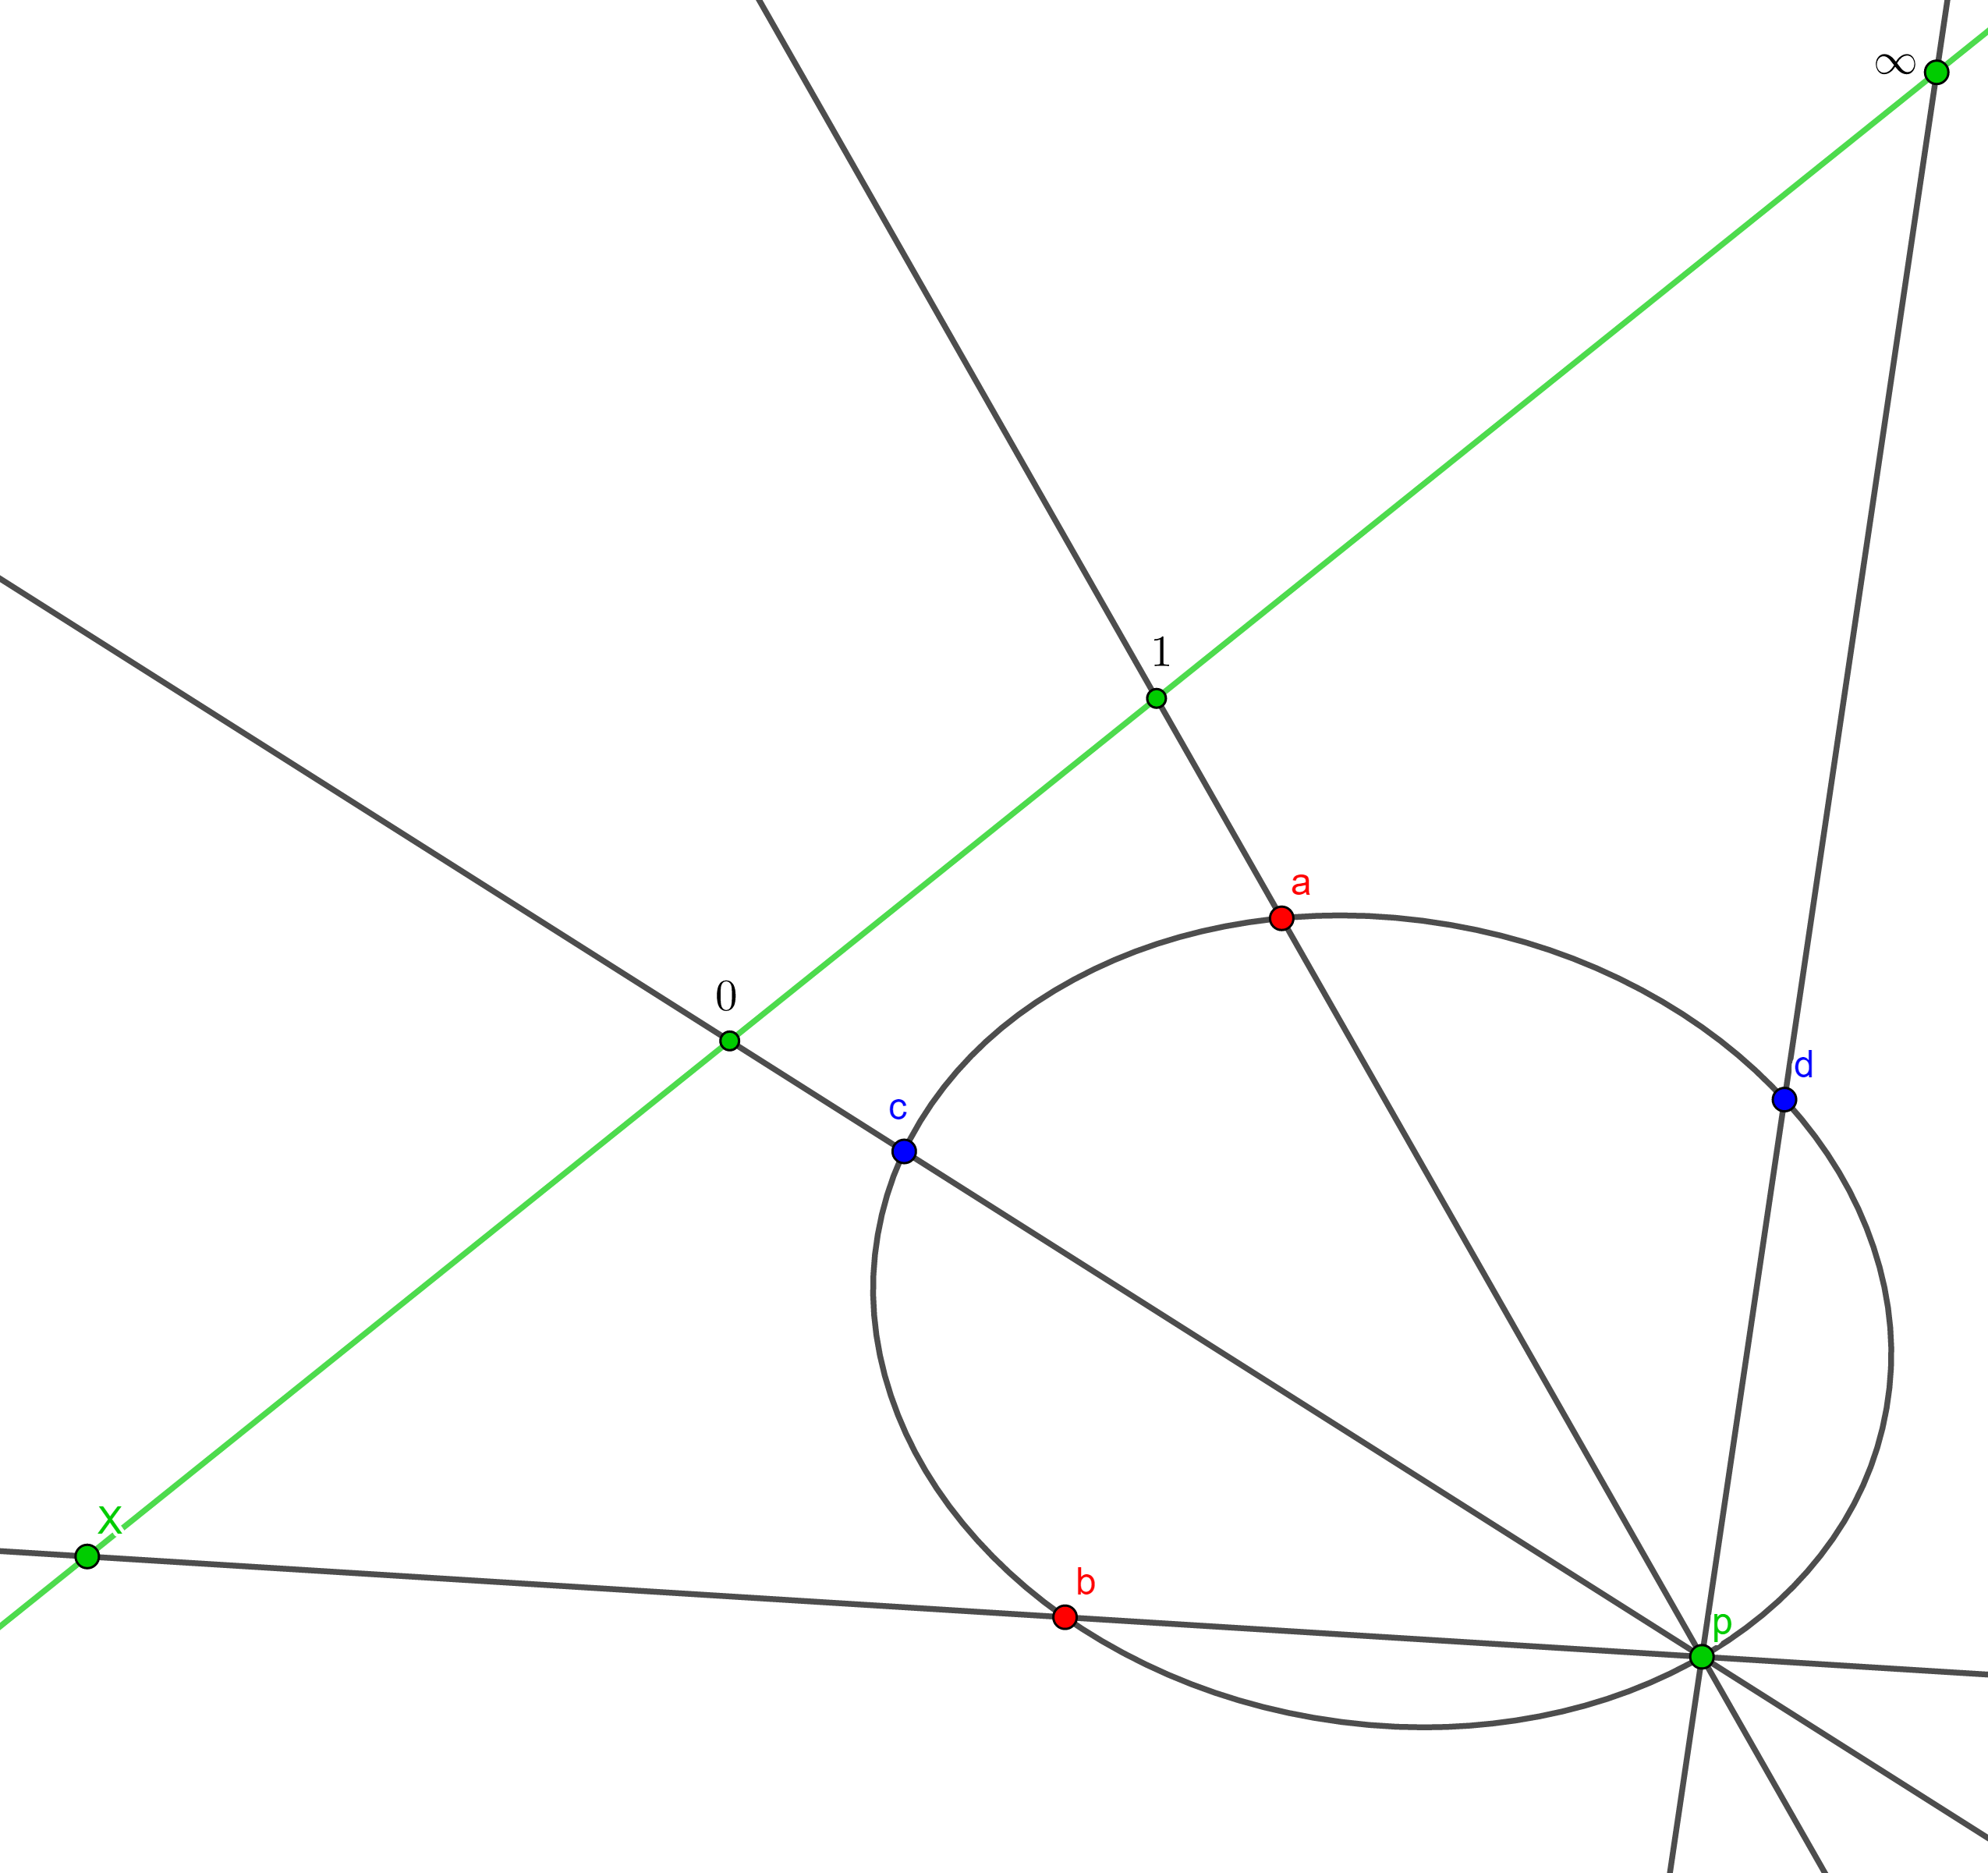
\includegraphics[width=0.5\linewidth]{pic19}
\end{figure}\\
$\sigma: (\infty, 0, 1, x) \rightarrow (0, \infty, 1, x)$, следовательно $[p_2, p_1, p_3, p_4] = [p_1, p_2, p_3, p_4]^{-1}$. Таким образом, $[a,b,c,d]=-1$\\

\vskip 0.2in
\noindent
\textbf{(б)}\\
Докажем, что поляра точки $P_3$ -- прямая $P_1P_2$. (Аналогично доказывается утверждение для точек $P_1$ и $P_2$.) \ \ $P_1P_2 \cup C = \{A, B\}$\\
$\{\text{id}, P_1, P_2, P_3\},\ P_i^2 = \text{id}$ -- группа Клейна, следовательно $P_1P_2=P_3$ и 
$\overbrace{P_2 \underbrace{P_1(A)}_{B}}^{A} = P_3(A)$, а значит $A=P_3(A)$.\\
Следовательно $P_3A, P_3B$ -- касательные к конике. Таким образом, $P_1P_2$ -- поляра $P_3$.\\
\begin{figure}[h!]
	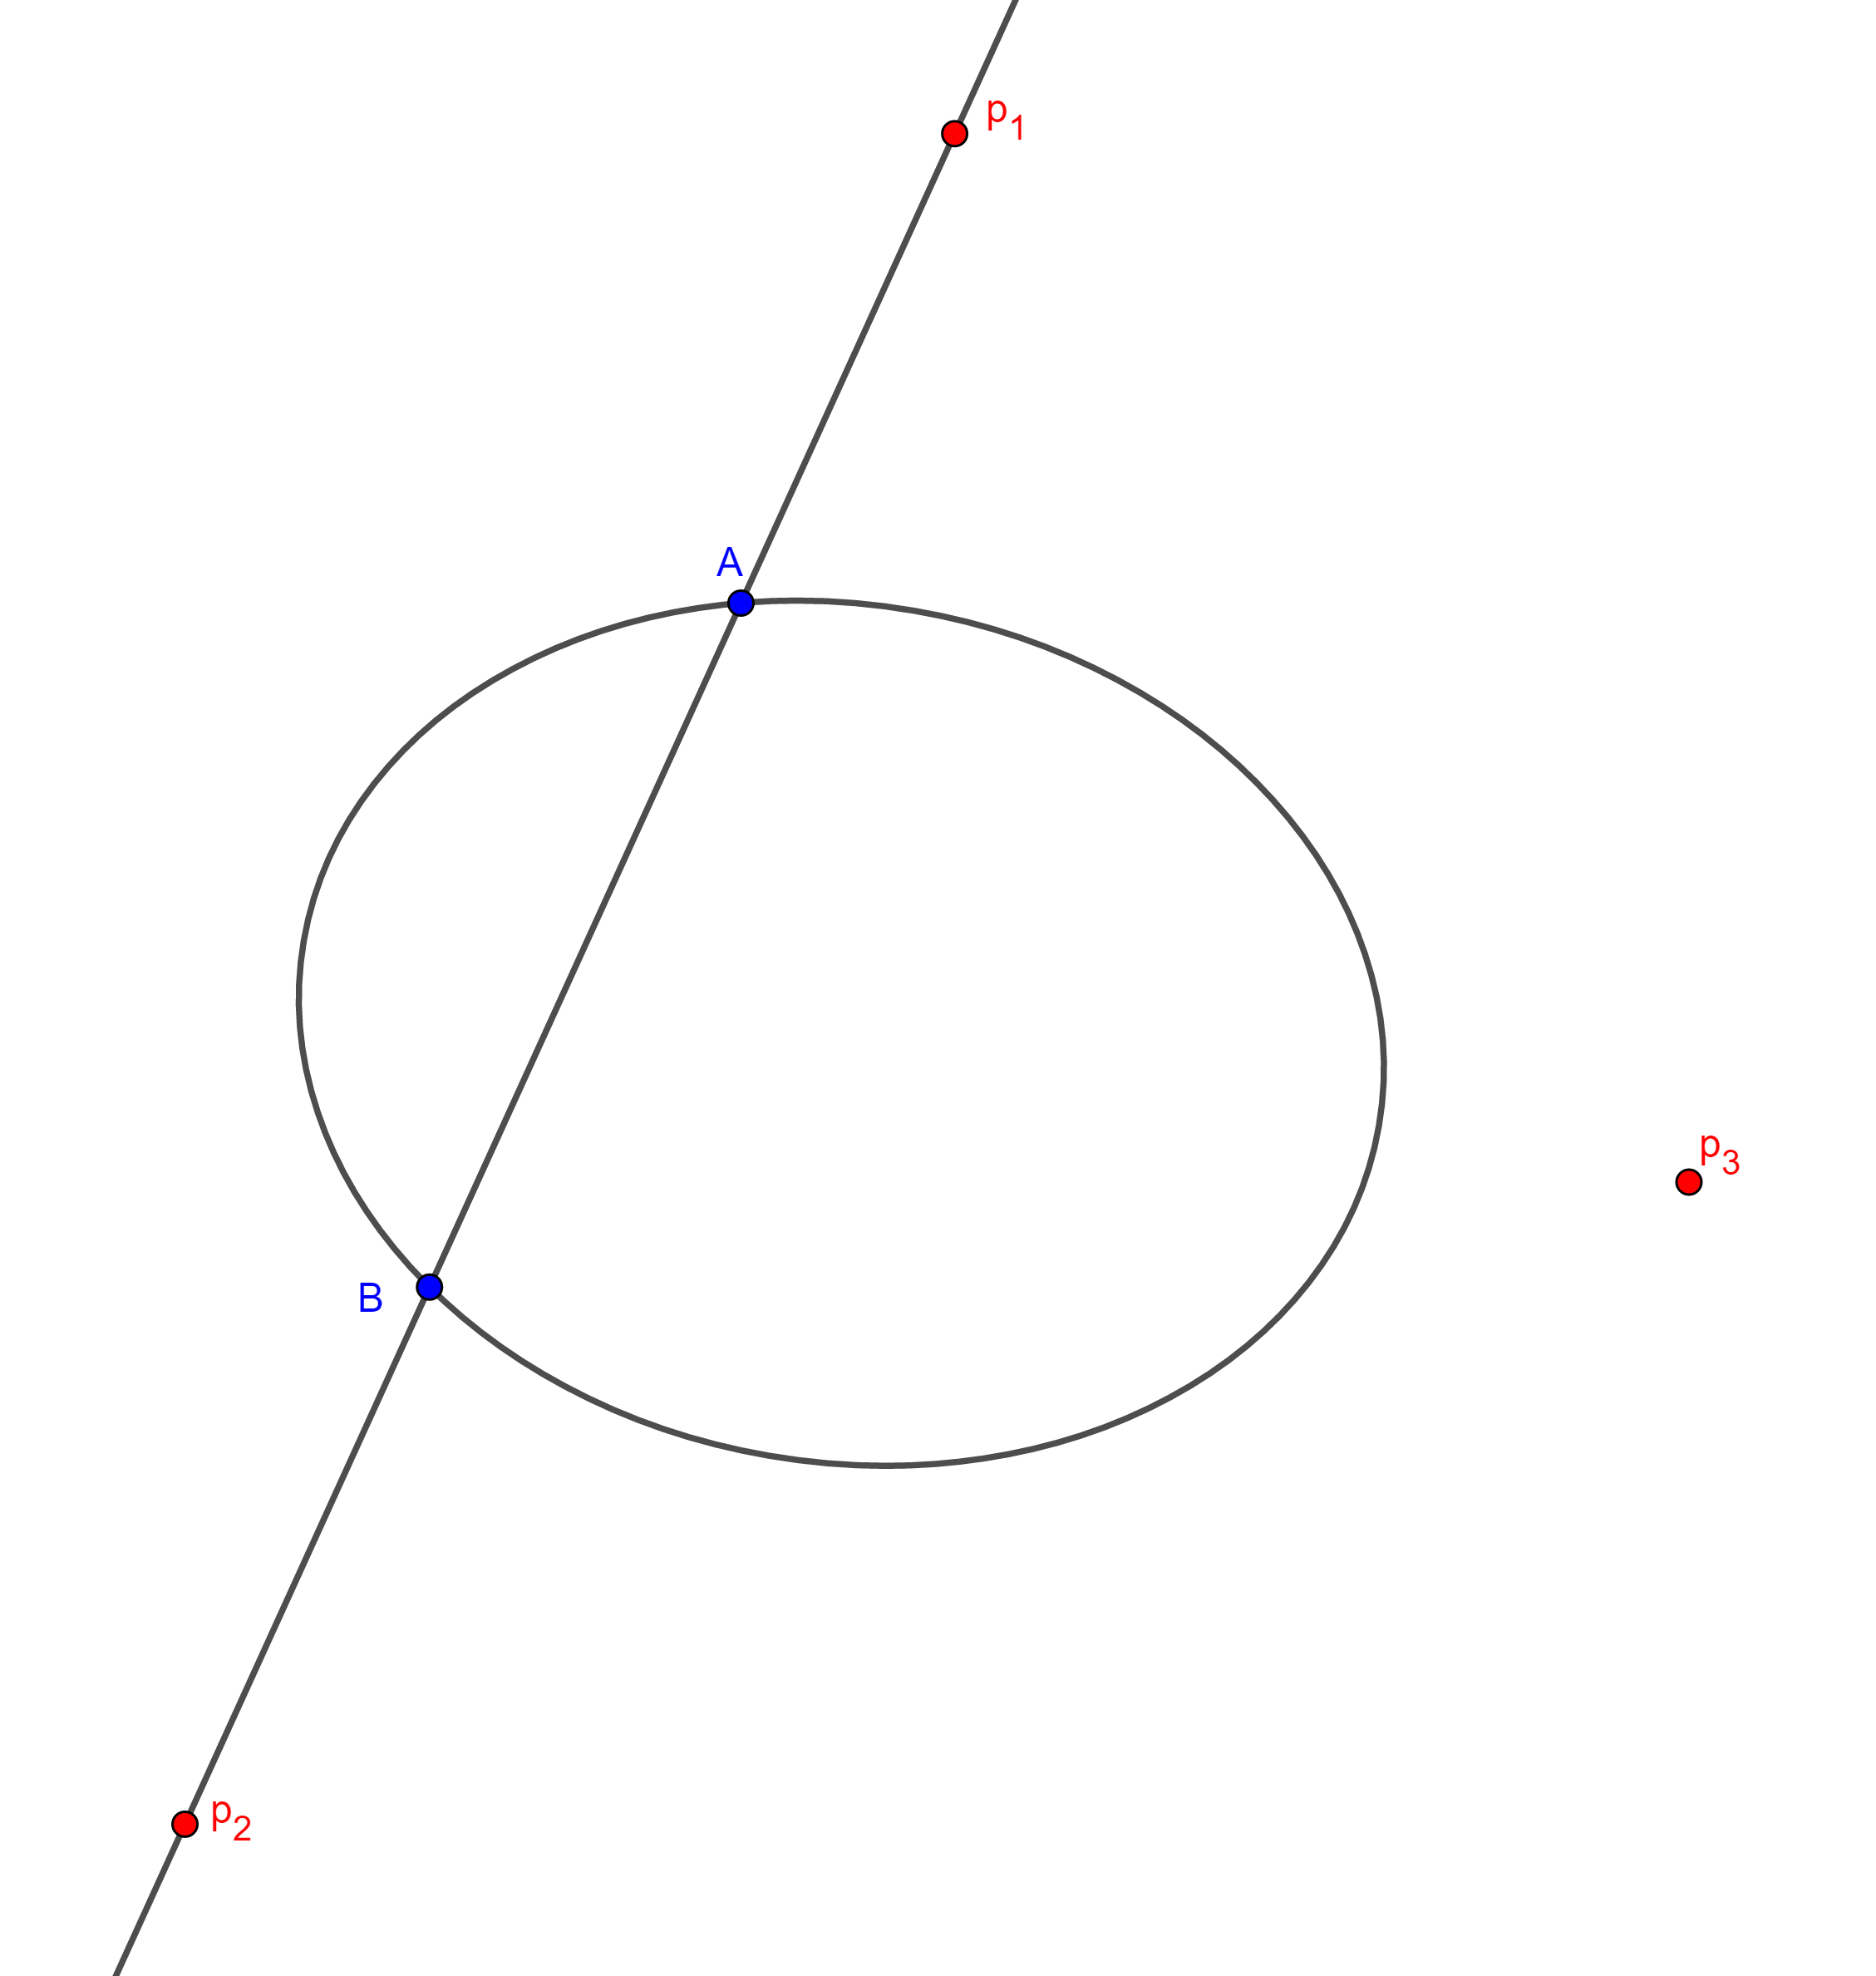
\includegraphics[width=0.45\linewidth]{pic20}
\end{figure}\\
		